\documentclass[solutions.tex]{subfiles}

\xtitle

\begin{document}
\maketitle
\begin{exercise} Verify the numerical values in each rap sheet.
\end{exercise}

\begin{remark} This is a long "solution": I'm taking the time to
rederive some results that were previously established either in
the course, or in earlier exercises, while, clarifying what I think
is a important source of confusion: the elements of an Hilbert space
(the so-called "state-space") \underline{aren't} the states of a
quantum system. More on that when exploring the singlet state. \\

Some numerical results have been automatically computed by a R script,
inlined at the end of this exercise.
\end{remark}

% All grouped and commented because it slows compilation time
% greatly. It could be managed more finely (e.g. without bashful,
% in the Makefile.
\iffalse
% I'm sure you can do this in pure LaTeX, but this is good enough.
%\iffalse
for (L in tau sigma) {
	for (d in x y z) {
		echo '\bash[stdoutFile=L07E12/'$L'_'$d'.tex]'
		echo 'Rscript L07E12.r '''$L'_'$d''' 2>/dev/null'
		echo '\END'
		echo ''
	}
}
%\fi

\bash[stdoutFile=L07E12/tau_x.tex]
Rscript L07E12.r 'tau_x' 2>/dev/null
\END

\bash[stdoutFile=L07E12/tau_y.tex]
Rscript L07E12.r 'tau_y' 2>/dev/null
\END

\bash[stdoutFile=L07E12/tau_z.tex]
Rscript L07E12.r 'tau_z' 2>/dev/null
\END

\bash[stdoutFile=L07E12/sigma_x.tex]
Rscript L07E12.r 'sigma_x' 2>/dev/null
\END

\bash[stdoutFile=L07E12/sigma_y.tex]
Rscript L07E12.r 'sigma_y' 2>/dev/null
\END

\bash[stdoutFile=L07E12/sigma_z.tex]
Rscript L07E12.r 'sigma_z' 2>/dev/null
\END

\bash[stdoutFile=L07E12/sigma_z-tau_z.tex]
Rscript L07E12.r 'sigma_z %*% tau_z' 2>/dev/null
\END

\bash[stdoutFile=L07E12/tau_z-sigma_z.tex]
Rscript L07E12.r 'tau_z %*% sigma_z' 2>/dev/null
\END

\bash[stdoutFile=L07E12/tau_x-sigma_x.tex]
Rscript L07E12.r 'tau_x %*% sigma_x' 2>/dev/null
\END

\bash[stdoutFile=L07E12/tau_y-sigma_y.tex]
Rscript L07E12.r 'tau_y %*% sigma_y' 2>/dev/null
\END

\bash[stdoutFile=L07E12/sigma_z-singlet.tex]
Rscript L07E12.r 'sigma_z' 0 '1/sqrt(2)' '-1/sqrt(2)' 0 2>/dev/null
\END
\bash[stdoutFile=L07E12/sigma_x-singlet.tex]
Rscript L07E12.r 'sigma_x' 0 '1/sqrt(2)' '-1/sqrt(2)' 0 2>/dev/null
\END
\bash[stdoutFile=L07E12/sigma_y-singlet.tex]
Rscript L07E12.r 'sigma_y' 0 '1/sqrt(2)' '-1/sqrt(2)' 0 2>/dev/null
\END

\bash[stdoutFile=L07E12/tau_z-singlet.tex]
Rscript L07E12.r 'tau_z' 0 '1/sqrt(2)' '-1/sqrt(2)' 0 2>/dev/null
\END
\bash[stdoutFile=L07E12/tau_x-singlet.tex]
Rscript L07E12.r 'tau_x' 0 '1/sqrt(2)' '-1/sqrt(2)' 0 2>/dev/null
\END
\bash[stdoutFile=L07E12/tau_y-singlet.tex]
Rscript L07E12.r 'tau_y' 0 '1/sqrt(2)' '-1/sqrt(2)' 0 2>/dev/null
\END

\bash[stdoutFile=L07E12/tau_z-sigma_z-singlet.tex]
Rscript L07E12.r 'tau_z %*% sigma_z' 0 '1/sqrt(2)' '-1/sqrt(2)' 0 2>/dev/null
\END
\bash[stdoutFile=L07E12/tau_x-sigma_x-singlet.tex]
Rscript L07E12.r 'tau_x %*% sigma_x' 0 '1/sqrt(2)' '-1/sqrt(2)' 0 2>/dev/null
\END
\bash[stdoutFile=L07E12/tau_y-sigma_y-singlet.tex]
Rscript L07E12.r 'tau_z %*% sigma_z' 0 '1/sqrt(2)' '-1/sqrt(2)' 0 2>/dev/null
\END

\bash[stdoutFile=L07E12/sigma_z-tau_z-singlet.tex]
Rscript L07E12.r 'sigma_z %*% tau_z' 0 '1/sqrt(2)' '-1/sqrt(2)' 0 2>/dev/null
\END

\bash[stdoutFile=L07E12/sigma_z-near-singlet.tex]
Rscript L07E12.r 'sigma_z' 0 'sqrt(0.6)' '-sqrt(0.4)' 0 2>/dev/null
\END
\bash[stdoutFile=L07E12/sigma_x-near-singlet.tex]
Rscript L07E12.r 'sigma_x' 0 'sqrt(0.6)' '-sqrt(0.4)' 0 2>/dev/null
\END
\bash[stdoutFile=L07E12/sigma_y-near-singlet.tex]
Rscript L07E12.r 'sigma_y' 0 'sqrt(0.6)' '-sqrt(0.4)' 0 2>/dev/null
\END

\bash[stdoutFile=L07E12/tau_z-near-singlet.tex]
Rscript L07E12.r 'tau_z' 0 'sqrt(0.6)' '-sqrt(0.4)' 0 2>/dev/null
\END
\bash[stdoutFile=L07E12/tau_x-near-singlet.tex]
Rscript L07E12.r 'tau_x' 0 'sqrt(0.6)' '-sqrt(0.4)' 0 2>/dev/null
\END
\bash[stdoutFile=L07E12/tau_y-near-singlet.tex]
Rscript L07E12.r 'tau_y' 0 'sqrt(0.6)' '-sqrt(0.4)' 0 2>/dev/null
\END

\bash[stdoutFile=L07E12/tau_z-sigma_z-near-singlet.tex]
Rscript L07E12.r 'tau_z %*% sigma_z' 0 'sqrt(0.6)' '-sqrt(0.4)' 0 2>/dev/null
\END
\bash[stdoutFile=L07E12/tau_x-sigma_x-near-singlet.tex]
Rscript L07E12.r 'tau_x %*% sigma_x' 0 'sqrt(0.6)' '-sqrt(0.4)' 0 2>/dev/null
\END
\bash[stdoutFile=L07E12/tau_y-sigma_y-near-singlet.tex]
Rscript L07E12.r 'tau_z %*% sigma_z' 0 'sqrt(0.6)' '-sqrt(0.4)' 0 2>/dev/null
\END

\bash[stdoutFile=L07E12/sigma_z-tau_z-near-singlet.tex]
Rscript L07E12.r 'sigma_z %*% tau_z' 0 'sqrt(0.6)' '-sqrt(0.4)' 0 2>/dev/null
\END
\fi

\hr

Let's start by recalling a few things before diving in. \\

We are, as usual, in the case of two spin systems, one for
Alice, $S_A$, one for Bob, $S_B$. A composite system $S_{AB}$
is then created from those two via a tensor product. \\

When relevant, we'll be using the usual ordered bases:
\begin{itemize}
	\item $\{\ket{u}, \ket{d}\}$ for $S_A$;
	\item $\{\keit{u}, \keit{d}\}$ for $S_B$;
	\item and $\{ \ket{uu}, \ket{ud}, \ket{du}, \ket{dd} \}$ for $S_{AB}$.
\end{itemize}

Then, let's recall the Pauli matrices corresponding to the
observables associated to the spin "components":
(from Eqs. $3.20$, at the end of section $3.4$)
\[
	\bm{\tau_z}^B = \bm{\sigma_z}^A = \begin{pmatrix}
		1 & 0 \\
		0 & -1 \\
	\end{pmatrix};\quad
	\bm{\tau_x}^B = \bm{\sigma_x}^A = \begin{pmatrix}
		0 & 1 \\
		1 & 0 \\
	\end{pmatrix};\quad
	\bm{\tau_y}^B = \bm{\sigma_y}^A = \begin{pmatrix}
		0 & -i \\
		i & 0 \\
	\end{pmatrix}
\]

Implicitly, the matrices are expressed in the ordered basis
of the corresponding sub-system, $S_A$ for $\bm{\sigma_i}^1$ and
$S_B$ for $\bm{\tau_i}^B$\footnote{Strictly speaking, the operators
aren't equal; their matrix representation in their respective-basis are.
The equals signs are to be understood in this context.}.
We will also need the matrix forms for the lifted operators from the
sub-systems to the composite system, where $\bm{I}^A$ is the identity
operator on $S_A$ and $\bm{I}^B$ the identity operator on $S_B$, again
implicitly relying on $S_{AB}$'s usual ordered basis. \\

\begin{remark} We could have used the equivalent tables provided
in annexes in the book, or the results of previous exercises.
\end{remark}

\begin{remark} Note that the final result appears twice below: this
isn't an error. The first occurence is a manual computation, while the
second has been automatically performed in \textit{R}.
\end{remark}

\begin{equation*}\begin{aligned}
	\bm{\sigma_z} &:=&& \bm{\sigma_z}^A\otimes\bm{I}^B &=&&
	\begin{pmatrix}
		1 & 0 \\
		0 & -1 \\
	\end{pmatrix}\otimes\begin{pmatrix}
		1 & 0 \\
		0 & 1 \\
	\end{pmatrix} &=&& \begin{pmatrix}
		1 & 0 & 0  & 0  \\
		0 & 1 & 0  & 0  \\
		0 & 0 & -1 & 0  \\
		0 & 0 & 0  & -1 \\
	\end{pmatrix} = % latex table generated in R 4.3.0 by xtable 1.8-4 package
% Thu Jun 15 10:20:36 2023
\begin{pmatrix}{}
  1 & 0 & 0 & 0 \\ 
  0 & 1 & 0 & 0 \\ 
  0 & 0 & -1 & 0 \\ 
  0 & 0 & 0 & -1 \\ 
  \end{pmatrix}
 \\
	\bm{\tau_z} &:=&& \bm{I}^A\otimes\bm{\tau_z}^B &=&&
	\begin{pmatrix}
		1 & 0 \\
		0 & 1 \\
	\end{pmatrix}\otimes\begin{pmatrix}
		1 & 0 \\
		0 & -1 \\
	\end{pmatrix} &=&& \begin{pmatrix}
		1 & 0  & 0 & 0  \\
		0 & -1 & 0 & 0  \\
		0 & 0  & 1 & 0  \\
		0 & 0  & 0 & -1 \\
	\end{pmatrix} = % latex table generated in R 4.3.0 by xtable 1.8-4 package
% Thu Jun 15 10:20:36 2023
\begin{pmatrix}{}
  1 & 0 & 0 & 0 \\ 
  0 & -1 & 0 & 0 \\ 
  0 & 0 & 1 & 0 \\ 
  0 & 0 & 0 & -1 \\ 
  \end{pmatrix}
 \\
\end{aligned}\end{equation*}
\begin{equation*}\begin{aligned}
	\bm{\sigma_x} &:=&& \bm{\sigma_x}^A\otimes\bm{I}^B &=&&
	\begin{pmatrix}
		0 & 1 \\
		1 & 0 \\
	\end{pmatrix}\otimes\begin{pmatrix}
		1 & 0 \\
		0 & 1 \\
	\end{pmatrix} &=&& \begin{pmatrix}
		0 & 0 & 1  & 0  \\
		0 & 0 & 0  & 1  \\
		1 & 0 & 0  & 0  \\
		0 & 1 & 0  & 0  \\
	\end{pmatrix} = % latex table generated in R 4.3.0 by xtable 1.8-4 package
% Thu Jun 15 10:20:36 2023
\begin{pmatrix}{}
  0 & 0 & 1 & 0 \\ 
  0 & 0 & 0 & 1 \\ 
  1 & 0 & 0 & 0 \\ 
  0 & 1 & 0 & 0 \\ 
  \end{pmatrix}
 \\
	\bm{\tau_x} &:=&& \bm{I}^A\otimes\bm{\tau_x}^B &=&&
	\begin{pmatrix}
		1 & 0 \\
		0 & 1 \\
	\end{pmatrix}\otimes\begin{pmatrix}
		0 & 1 \\
		1 & 0 \\
	\end{pmatrix} &=&& \begin{pmatrix}
		0 & 1 & 0  & 0  \\
		1 & 0 & 0  & 0  \\
		0 & 0 & 0  & 1  \\
		0 & 0 & 1  & 0  \\
	\end{pmatrix}  = % latex table generated in R 4.3.0 by xtable 1.8-4 package
% Thu Jun 15 10:20:35 2023
\begin{pmatrix}{}
  0 & 1 & 0 & 0 \\ 
  1 & 0 & 0 & 0 \\ 
  0 & 0 & 0 & 1 \\ 
  0 & 0 & 1 & 0 \\ 
  \end{pmatrix}
\\
\end{aligned}\end{equation*}
\begin{equation*}\begin{aligned}
	\bm{\sigma_y} &:=&& \bm{\sigma_y}^A\otimes\bm{I}^B &=&&
	\begin{pmatrix}
		0 & -i \\
		i & 0 \\
	\end{pmatrix}\otimes\begin{pmatrix}
		1 & 0 \\
		0 & 1 \\
	\end{pmatrix} &=&& \begin{pmatrix}
		0 & 0 & -i  & 0  \\
		0 & 0 & 0  & -i  \\
		i & 0 & 0  & 0  \\
		0 & i & 0  & 0  \\
	\end{pmatrix} = % latex table generated in R 4.3.0 by xtable 1.8-4 package
% Thu Jun 15 10:20:36 2023
\begin{pmatrix}{}
  0 & 0 &  -i & 0 \\ 
  0 & 0 & 0 &  -i \\ 
   i & 0 & 0 & 0 \\ 
  0 &  i & 0 & 0 \\ 
  \end{pmatrix}
 \\
	\bm{\tau_y} &:=&& \bm{I}^A\otimes\bm{\tau_y}^B &=&&
	\begin{pmatrix}
		1 & 0 \\
		0 & 1 \\
	\end{pmatrix}\otimes\begin{pmatrix}
		0 & -i \\
		i & 0 \\
	\end{pmatrix} &=&& \begin{pmatrix}
		0 & -i & 0  & 0  \\
		i & 0 & 0  & 0  \\
		0 & 0 & 0  & -i  \\
		0 & 0 & i  & 0  \\
	\end{pmatrix} = % latex table generated in R 4.3.0 by xtable 1.8-4 package
% Thu Jun 15 10:20:35 2023
\begin{pmatrix}{}
  0 &  -i & 0 & 0 \\ 
   i & 0 & 0 & 0 \\ 
  0 & 0 & 0 &  -i \\ 
  0 & 0 &  i & 0 \\ 
  \end{pmatrix}
 \\
\end{aligned}\end{equation*}

We'll also need a few more "combined" observables. I'll skip the manual
matrix multiplication here: those have been automatically computed
by \textit{R}:

\[
	\bm{\sigma_z}\bm{\tau_z} = % latex table generated in R 4.3.0 by xtable 1.8-4 package
% Thu Jun 15 10:20:37 2023
\begin{pmatrix}{}
  1 & 0 & 0 & 0 \\ 
  0 & -1 & 0 & 0 \\ 
  0 & 0 & -1 & 0 \\ 
  0 & 0 & 0 & 1 \\ 
  \end{pmatrix}
;\qquad
	\bm{\tau_z}\bm{\sigma_z} = % latex table generated in R 4.3.0 by xtable 1.8-4 package
% Thu Jun 15 10:20:37 2023
\begin{pmatrix}{}
  1 & 0 & 0 & 0 \\ 
  0 & -1 & 0 & 0 \\ 
  0 & 0 & -1 & 0 \\ 
  0 & 0 & 0 & 1 \\ 
  \end{pmatrix}

\]

\[
	\bm{\tau_x}\bm{\sigma_x} = % latex table generated in R 4.3.0 by xtable 1.8-4 package
% Thu Jun 15 10:20:37 2023
\begin{pmatrix}{}
  0 & 0 & 0 & 1 \\ 
  0 & 0 & 1 & 0 \\ 
  0 & 1 & 0 & 0 \\ 
  1 & 0 & 0 & 0 \\ 
  \end{pmatrix}
;\qquad
	\bm{\tau_y}\bm{\sigma_y} = % latex table generated in R 4.3.0 by xtable 1.8-4 package
% Thu Jun 15 10:20:37 2023
\begin{pmatrix}{}
  0 & 0 & 0 & -1 \\ 
  0 & 0 & 1 & 0 \\ 
  0 & 1 & 0 & 0 \\ 
  -1 & 0 & 0 & 0 \\ 
  \end{pmatrix}

\]


Finally, let's recall one more time the formula for the expectation value
$\avg{\bm{L}}$ of an observable $\bm{L}$ of a system in a state $\ket{\Psi}$:
\[
	\avg{\bm{L}} = \bra{\Psi}\bm{L}\ket{\Psi}
\]

\hr

\textbf{Product state}\ \\

We're starting from the following state-vector for the composite
system, and using various properties of the tensor product of
vector states we progressively reach:
\begin{equation*}\begin{aligned}
	\ket{\Psi} &=&& \alpha_u\beta_u\ket{uu}
		+\alpha_u\beta_d\ket{ud}
		+\alpha_d\beta_u\ket{du}
		+\alpha_d\beta_d\ket{dd} \\
	~ &=&& \alpha_u\beta_u\ket{u}\otimes\keit{u}
		+\alpha_u\beta_d\ket{u}\otimes\keit{d}
		+\alpha_d\beta_u\ket{d}\otimes\keit{u}
		+\alpha_d\beta_d\ket{d}\otimes\keit{d} \\
	~ &=&& (\alpha_u\ket{u})\otimes(\beta_u\keit{u})
		+(\alpha_u\ket{u})\otimes(\beta_d\keit{d})
		+(\alpha_d\ket{d})\otimes(\beta_u\keit{u})
		+(\alpha_d\ket{d})\otimes(\beta_d\keit{d}) \\
	~ &=&& \alpha_u\ket{u}\otimes(\beta_d\keit{d} + \beta_u\keit{u})
		+ \alpha_d\ket{d}\otimes(\beta_u\keit{u} + \beta_d\keit{d}) \\
	~ &=&& \underbrace{(\alpha_u\ket{u}+ \alpha_d\ket{d})}_{=:\ket{\phi}}
		\otimes\underbrace{(\beta_d\keit{d} + \beta_u\keit{u})}_{=:\keit{\psi}} \\
\end{aligned}\end{equation*}

We've verified that this particular composite state is a
\underline{state product}: it can be expressed as the tensor product of
two states, $\ket{\phi}\in S_A$ and $\keit{\psi}\in S_B$. \\

The \underline{normalization condition} yields:
\begin{equation*}\begin{aligned}
	\norm{\ket{\Psi}} := \sqrt{\braket{\Psi}{\Psi}} =1 &\Leftrightarrow &&
		\sqrt{
			\alpha_u^*\beta_u^*\alpha_u\beta_u
			+\alpha_u^*\beta_d^*\alpha_u\beta_d
			+\alpha_d^*\beta_u^*\alpha_d\beta_u
			+\alpha_d^*\beta_d^*\alpha_d\beta_d
		} = 1 \\
	~ &\Leftrightarrow&&
		\sqrt{
			\alpha_u^*\alpha_u(\beta_u^*\beta_u+\beta_d^*\beta_d)
			+\alpha_d^*\alpha_d(\beta_u^*\beta_u+\beta_d^*\beta_d)
		} = 1 \\
	~ &\Leftrightarrow&&
		\sqrt{
			(\alpha_u^*\alpha_u+\alpha_d^*\alpha_d)
			(\beta_u^*\beta_u+\beta_d^*\beta_d)
		} = 1 \\
	~ &\Leftrightarrow&&
		(\alpha_u^*\alpha_u+\alpha_d^*\alpha_d)
		(\beta_u^*\beta_u+\beta_d^*\beta_d) = 1 &
			(\forall\gamma\in\mathbb{C}),\,\gamma^*\gamma=:|\gamma| > 0 \\
	~ &\Leftrightarrow&&
		\begin{cases}
			\alpha_u^*\alpha_u+\alpha_d^*\alpha_d &= 1 \\
			\beta_u^*\beta_u+\beta_d^*\beta_d &= 1 \\
		\end{cases} \\
	~ &\Leftrightarrow&&
		\begin{cases}
			\sqrt{\alpha_u^*\alpha_u+\alpha_d^*\alpha_d} &= 1 \\
			\sqrt{\beta_u^*\beta_u+\beta_d^*\beta_d} &= 1 \\
		\end{cases}&
			(\forall\gamma\in\mathbb{C}),\,\gamma^*\gamma=:|\gamma| > 0 \\
	~ &\Leftrightarrow&&
		\begin{cases}
			\norm{\ket{\phi}} &= 1 \\
			\norm{\keit{\psi}} &= 1 \\
		\end{cases} \\
\end{aligned}\end{equation*}

We've verified consistency of the normalization condition
between the composite system, and the sub-systems: our composite state vector
is normalized iff the individual vectors from the sub-systems are
normalized. \\

Moving on to the \underline{density matrices}, let's do the reasoning
for Alice's state only, as the same argument applies to Bob's. Let's
first stay in $S_A$. We know that the subsystem's state
is a \textit{pure} state $\ket{\phi}$: it's a convex combination%
\footnote{\url{https://en.wikipedia.org/wiki/Convex\_combination}} with
a single term. The density matrix $\rho^A$ is thus:
\[
	\rho^A = 1\ket{\phi}\bra{\phi} = \begin{pmatrix}
		\alpha_u \\
		\alpha_d \\
	\end{pmatrix}\begin{pmatrix}
		\alpha_u^* & \alpha_d^* \\
	\end{pmatrix} = \begin{pmatrix}
		\alpha_u\alpha_u^* & \alpha_u\alpha_d^* \\
		\alpha_d\alpha_u^* & \alpha_d\alpha_d^* \\
	\end{pmatrix}
\]

It is immediate to check that $\rho^A$ is Hermitian ($\rho^A = (\rho^A)^\dagger$,
as $(\alpha_u\alpha_d^*)^* = \alpha_d\alpha_u^*$).
Furthermore:
\[
	\Tr(\rho^A) = \alpha_u\alpha_u^* + \alpha_d\alpha_d^* = 1
	\text{ (because of the normalization condition)}
\]

We also have:
\begin{equation*}\begin{aligned}
	(\rho^A)^2 &=&&  \begin{pmatrix}
		\alpha_u\alpha_u^* & \alpha_u\alpha_d^* \\
		\alpha_d\alpha_u^* & \alpha_d\alpha_d^* \\
	\end{pmatrix} \begin{pmatrix}
		\alpha_u\alpha_u^* & \alpha_u\alpha_d^* \\
		\alpha_d\alpha_u^* & \alpha_d\alpha_d^* \\
	\end{pmatrix} \\
	~ &=&& \begin{pmatrix}
		(\alpha_u\alpha_u^*)(\alpha_u\alpha_u^*)
		+(\alpha_u\alpha_d^*)(\alpha_d\alpha_u^*)
		&
		(\alpha_u\alpha_u^*)(\alpha_u\alpha_d^*)
		+ (\alpha_u\alpha_d^*)(\alpha_d\alpha_d^*)
		\\
		(\alpha_d\alpha_u^*)(\alpha_u\alpha_u^*)
		+(\alpha_d\alpha_d^*)(\alpha_d\alpha_u^*)
		&
		(\alpha_d\alpha_u^*)(\alpha_u\alpha_d^*)
		+(\alpha_d\alpha_d^*)(\alpha_d\alpha_d^*)
		\\
	\end{pmatrix} \\
	~ &=&& \begin{pmatrix}
		(\alpha_u\alpha_u^*)\underbrace{
			(\alpha_u\alpha_u^* + \alpha_d^*\alpha_d)
		}_{=1}
		&
		(\alpha_u\alpha_d^*)\underbrace{
			(\alpha_u\alpha_u^* + \alpha_d^*\alpha_d)
		}_{=1}
		\\
		(\alpha_d\alpha_u^*)\underbrace{
			(\alpha_u\alpha_u^* + \alpha_d^*\alpha_d)
		}_{=1}
		&
		(\alpha_d\alpha_d^*)\underbrace{
			(\alpha_u\alpha_u^* + \alpha_d^*\alpha_d)
		}_{=1}
		\\
	\end{pmatrix} \\
	~ &=&& \rho^A \\
\end{aligned}\end{equation*}

And naturally, $\Tr((\rho^A)^2) = \Tr(\rho) = 1$. Those last two conditions
are indeed we expect for a pure state. \\

Let's move on to diagonalizing $\rho^A$. As usual, eigenvectors $\ket{\lambda}$
are tied to their corresponding eigenvalues $\lambda$ via:
\begin{equation*}\begin{aligned}
	\rho^A\ket{\lambda} = \lambda\ket{\lambda}
	\Leftrightarrow
	(\rho^A-\bm{I}^A\lambda)\ket{\lambda} = 0
	&\Leftrightarrow&&
	|\rho^A-\bm{I}^A\lambda| = 0 \\
	~&\Leftrightarrow&&
	\begin{vmatrix}
		\alpha_u\alpha_u^*-\lambda & \alpha_u\alpha_d^* \\
		\alpha_d\alpha_u^* & \alpha_d\alpha_d^*-\lambda \\
	\end{vmatrix} \\
	~&\Leftrightarrow&&
	(\alpha_u\alpha_u^*-\lambda)(\alpha_d\alpha_d^*-\lambda)
	-\alpha_d\alpha_u^*\alpha_u\alpha_d^* = 0\\
	~&\Leftrightarrow&&
	\lambda^2-\underbrace{(\alpha_u\alpha_u^*+\alpha_d\alpha_d^*)}_{=1}\lambda = 0 \\
	~&\Leftrightarrow&&
	\lambda(\lambda-1) = 0 \\
	~&\Leftrightarrow&&
	\begin{cases}
		\lambda &= 0 \\
		\lambda &= 1 \\
	\end{cases}
\end{aligned}\end{equation*}

Let's verify that the eigenvector $\ket{\lambda_1}$ associated to $\lambda=1$
is indeed the wave-function associated to Alice's sub-system, i.e with
components $\alpha_u$ and $\alpha_d$
\[
	\rho^A\ket{\lambda_1} = \begin{pmatrix}
		\alpha_u\alpha_u^* & \alpha_u\alpha_d^* \\
		\alpha_d\alpha_u^* & \alpha_d\alpha_d^* \\
	\end{pmatrix}\begin{pmatrix}
		\alpha_u \\
		\beta_d \\
	\end{pmatrix} = \begin{pmatrix}
		\alpha_u\alpha_u^*\alpha_u + \alpha_u\alpha_d^*\alpha_d \\
		\alpha_d\alpha_u^*\alpha_u + \alpha_d\alpha_d^*\alpha_d \\
	\end{pmatrix} = \begin{pmatrix}
		\alpha_u\underbrace{(\alpha_u^*\alpha_u+\alpha_d^*\alpha_d)}_{=1} \\
		\alpha_d\underbrace{(\alpha_u^*\alpha_u+\alpha_d^*\alpha_d)}_{=1} \\
	\end{pmatrix} = 1\ket{\lambda_1}
\]

Again, by symmetry, we immediately have for $S_B$:
\[
	\rho_B = \begin{pmatrix}
		\beta_u\beta_u^* & \beta_u\beta_d^* \\
		\beta_d\beta_u^* & \beta_d\beta_d^* \\
	\end{pmatrix};\qquad
	\rho_B^2 = \rho_B;\qquad \Tr(\rho_B^2) = \Tr(\rho_B) = 1
\]

Same eigenvalues/eigenvectors. \\

What about $S_{AB}$? Well, $\ket{\Psi}$ still is a pure state in $S_{AB}$,
meaning, its density matrix again is a convex combination involving
a single term; expanding it as a matrix in $S_{AB}$'s usual ordered basis
yields:
\begin{equation*}\begin{aligned}
	\rho = 1\ket{\Psi}\bra{\Psi} &=&& \begin{pmatrix}
		\alpha_u\beta_u \\
		\alpha_u\beta_d \\
		\alpha_d\beta_u \\
		\alpha_d\beta_d \\
	\end{pmatrix}\begin{pmatrix}
		(\alpha_u\beta_u)^* & (\alpha_u\beta_d)^* &
			(\alpha_d\beta_u)^* + (\alpha_d\beta_d)^*
	\end{pmatrix} \\
	~ &=&& \begin{pmatrix}
		\alpha_u\beta_u\alpha_u^*\beta_u^*
			& \alpha_u\beta_u\alpha_u^*\beta_d^*
			& \alpha_u\beta_u\alpha_d^*\beta_u^*
			& \alpha_u\beta_u\alpha_d^*\beta_d^* \\
		\alpha_u\beta_d\alpha_u^*\beta_u^*
			& \alpha_u\beta_d\alpha_u^*\beta_d^*
			& \alpha_u\beta_d\alpha_d^*\beta_u^*
			& \alpha_u\beta_d\alpha_d^*\beta_d^* \\
		\alpha_d\beta_u\alpha_u^*\beta_u^*
			& \alpha_d\beta_u\alpha_u^*\beta_d^*
			& \alpha_d\beta_u\alpha_d^*\beta_u^*
			& \alpha_d\beta_u\alpha_d^*\beta_d^* \\
		\alpha_d\beta_d\alpha_u^*\beta_u^*
			& \alpha_d\beta_d\alpha_u^*\beta_d^*
			& \alpha_d\beta_d\alpha_d^*\beta_u^*
			& \alpha_d\beta_d\alpha_d^*\beta_d^* \\
	\end{pmatrix} \\
\end{aligned}\end{equation*}

Because this is again a pure state, this time in the $S_{AB}$ system,
we expect the usual formulas to hold. Let's check them for good measure:
\begin{equation*}\begin{aligned}
	\Tr(\rho) &=&& \alpha_u\beta_u\alpha_u^*\beta_u^*
		+ \alpha_u\beta_d\alpha_u^*\beta_d^*
		+ \alpha_d\beta_u\alpha_d^*\beta_u^*
		+ \alpha_d\beta_d\alpha_d^*\beta_d^* \\
	~ &=&& \alpha_u\alpha_u^*\underbrace{(
		\beta_u\beta_u^* + \beta_d\beta_d^*
	)}_{=1} + \alpha_d\alpha_d^*\underbrace{(
		\beta_u\beta_u^*+ \beta_d\beta_d^*
	)}_{=1} \\
	~ &=&& 1 \\
\end{aligned}\end{equation*}

The following is going to be too tedious to do by hand:
\begin{equation*}\begin{aligned}
	\rho^2 &=&& \begin{pmatrix}
		\alpha_u\beta_u\alpha_u^*\beta_u^*
			& \alpha_u\beta_u\alpha_u^*\beta_d^*
			& \alpha_u\beta_u\alpha_d^*\beta_u^*
			& \alpha_u\beta_u\alpha_d^*\beta_d^* \\
		\alpha_u\beta_d\alpha_u^*\beta_u^*
			& \alpha_u\beta_d\alpha_u^*\beta_d^*
			& \alpha_u\beta_d\alpha_d^*\beta_u^*
			& \alpha_u\beta_d\alpha_d^*\beta_d^* \\
		\alpha_d\beta_u\alpha_u^*\beta_u^*
			& \alpha_d\beta_u\alpha_u^*\beta_d^*
			& \alpha_d\beta_u\alpha_d^*\beta_u^*
			& \alpha_d\beta_u\alpha_d^*\beta_d^* \\
		\alpha_d\beta_d\alpha_u^*\beta_u^*
			& \alpha_d\beta_d\alpha_u^*\beta_d^*
			& \alpha_d\beta_d\alpha_d^*\beta_u^*
			& \alpha_d\beta_d\alpha_d^*\beta_d^* \\
	\end{pmatrix}\begin{pmatrix}
		\alpha_u\beta_u\alpha_u^*\beta_u^*
			& \alpha_u\beta_u\alpha_u^*\beta_d^*
			& \alpha_u\beta_u\alpha_d^*\beta_u^*
			& \alpha_u\beta_u\alpha_d^*\beta_d^* \\
		\alpha_u\beta_d\alpha_u^*\beta_u^*
			& \alpha_u\beta_d\alpha_u^*\beta_d^*
			& \alpha_u\beta_d\alpha_d^*\beta_u^*
			& \alpha_u\beta_d\alpha_d^*\beta_d^* \\
		\alpha_d\beta_u\alpha_u^*\beta_u^*
			& \alpha_d\beta_u\alpha_u^*\beta_d^*
			& \alpha_d\beta_u\alpha_d^*\beta_u^*
			& \alpha_d\beta_u\alpha_d^*\beta_d^* \\
		\alpha_d\beta_d\alpha_u^*\beta_u^*
			& \alpha_d\beta_d\alpha_u^*\beta_d^*
			& \alpha_d\beta_d\alpha_d^*\beta_u^*
			& \alpha_d\beta_d\alpha_d^*\beta_d^* \\
	\end{pmatrix} \\
	~ &=&& \ldots \\
	~ &=&& \rho \\
\end{aligned}\end{equation*}

With some text reformatting and a few tweak, we can convert the \LaTeX
code in a Wolfram Alpha matrix:
\begin{verbatim}
{{a c Conjugate(a) Conjugate(c),a c Conjugate(a) Conjugate(d),
    a c Conjugate(b) Conjugate(c),
    a c Conjugate(b) Conjugate(d)},
{a d Conjugate(a) Conjugate(c),
    a d Conjugate(a) Conjugate(d),
    a d Conjugate(b) Conjugate(c),
    a d Conjugate(b) Conjugate(d)},
{b c Conjugate(a) Conjugate(c),
    b c Conjugate(a) Conjugate(d),
    b c Conjugate(b) Conjugate(c),
    b c Conjugate(b) Conjugate(d)},
{b d Conjugate(a) Conjugate(c),
    b d Conjugate(a) Conjugate(d),
    b d Conjugate(b) Conjugate(c),
    b d Conjugate(b) Conjugate(d)}}
\end{verbatim}

And use for instance the web interface (see \url{https://www.wolframalpha.com/input?i2d=true&i=Power%5B%7B%7Ba+c+Conjugate%5C%2840%29a%5C%2841%29+Conjugate%5C%2840%29c%5C%2841%29%2Ca+c+Conjugate%5C%2840%29a%5C%2841%29+Conjugate%5C%2840%29d%5C%2841%29%2Ca+c+Conjugate%5C%2840%29b%5C%2841%29+Conjugate%5C%2840%29c%5C%2841%29%2Ca+c+Conjugate%5C%2840%29b%5C%2841%29+Conjugate%5C%2840%29d%5C%2841%29%7D%2C%7Ba+d+Conjugate%5C%2840%29a%5C%2841%29+Conjugate%5C%2840%29c%5C%2841%29%2Ca+d+Conjugate%5C%2840%29a%5C%2841%29+Conjugate%5C%2840%29d%5C%2841%29%2Ca+d+Conjugate%5C%2840%29b%5C%2841%29+Conjugate%5C%2840%29c%5C%2841%29%2Ca+d+Conjugate%5C%2840%29b%5C%2841%29+Conjugate%5C%2840%29d%5C%2841%29%7D%2C%7Bb+c+Conjugate%5C%2840%29a%5C%2841%29+Conjugate%5C%2840%29c%5C%2841%29%2Cb+c+Conjugate%5C%2840%29a%5C%2841%29+Conjugate%5C%2840%29d%5C%2841%29%2Cb+c+Conjugate%5C%2840%29b%5C%2841%29+Conjugate%5C%2840%29c%5C%2841%29%2Cb+c+Conjugate%5C%2840%29b%5C%2841%29+Conjugate%5C%2840%29d%5C%2841%29%7D%2C%7Bb+d+Conjugate%5C%2840%29a%5C%2841%29+Conjugate%5C%2840%29c%5C%2841%29%2Cb+d+Conjugate%5C%2840%29a%5C%2841%29+Conjugate%5C%2840%29d%5C%2841%29%2Cb+d+Conjugate%5C%2840%29b%5C%2841%29+Conjugate%5C%2840%29c%5C%2841%29%2Cb+d+Conjugate%5C%2840%29b%5C%2841%29+Conjugate%5C%2840%29d%5C%2841%29%7D%7D%2C2%5D})
to make sure it works:

\begin{figure}[H]
	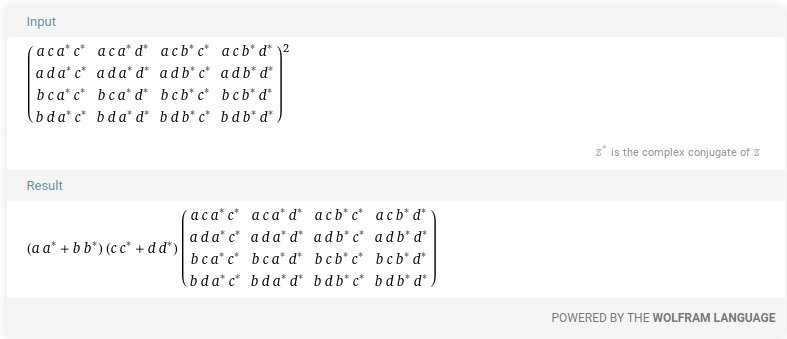
\includegraphics[width=\textwidth]{rho_square_wolfram.jpg}
	\centering
\end{figure}
\begin{remark} The leading factors correspond to the norms of
the sub-system states: it's a $1$ in disguise.
\end{remark}

It follows that $\Tr(\rho^2) = \Tr(\rho) = 1$. \\

We've already brushed upon it, but let's make things crystal clear regarding
the \underline{wave-functions}: we have one wave function for each sub-systems:
\begin{equation*}\begin{aligned}
	\psi^A(\ket{u}) &=&& \alpha_u;&&&\psi^B(\keit{u}) = \beta_u; \\
	\psi^A(\ket{d}) &=&& \alpha_d;&&&\psi^B(\keit{d}) = \beta_d. \\
\end{aligned}\end{equation*}

And a wave-function for the composite system, which indeed factorize as
a product of the sub-systems wave-functions:
\[
	\psi : \begin{cases}
		\ket{uu} &\rightarrow \alpha_u\beta_u = \psi^A(\ket{u})\psi^B(\keit{u}) \\
		\ket{ud} &\rightarrow \alpha_u\beta_d = \psi^A(\ket{u})\psi^B(\keit{d}) \\
		\ket{du} &\rightarrow \alpha_d\beta_u = \psi^A(\ket{d})\psi^B(\keit{u}) \\
		\ket{dd} &\rightarrow \alpha_d\beta_d = \psi^A(\ket{d})\psi^B(\keit{d}) \\
	\end{cases} \Leftrightarrow \psi(a,b) = \psi^A(a)\psi^B(b)
\]

Finally, we can crunch some numbers using the usual expectation value
formula, using the matrices for the spin observables we've re-established
earlier. This could have been automated, but I haven't looked much into
how to perform symbolic computation with R.

\begin{equation*}\begin{aligned}
	\avg{\bm{\sigma_x}} = \bra{\Psi}\bm{\sigma_x}\ket{\Psi}
		&=&& \begin{pmatrix}
			\alpha_u^*\beta_u^* &
			\alpha_u^*\beta_d^* &
			\alpha_d^*\beta_u^* &
			\alpha_d^*\beta_d^* &
		\end{pmatrix}% latex table generated in R 4.3.0 by xtable 1.8-4 package
% Thu Jun 15 10:20:36 2023
\begin{pmatrix}{}
  0 & 0 & 1 & 0 \\ 
  0 & 0 & 0 & 1 \\ 
  1 & 0 & 0 & 0 \\ 
  0 & 1 & 0 & 0 \\ 
  \end{pmatrix}
\begin{pmatrix}
			\alpha_u\beta_u \\
			\alpha_u\beta_d \\
			\alpha_d\beta_u \\
			\alpha_d\beta_d \\
		\end{pmatrix} \\
	~ &=&& \begin{pmatrix}
			\alpha_u^*\beta_u^* &
			\alpha_u^*\beta_d^* &
			\alpha_d^*\beta_u^* &
			\alpha_d^*\beta_d^* &
		\end{pmatrix}\begin{pmatrix}
			\alpha_d\beta_u \\
			\alpha_d\beta_d \\
			\alpha_u\beta_u \\
			\alpha_u\beta_d \\
		\end{pmatrix} \\
	~ &=&& \alpha_u^*\beta_u^*\alpha_d\beta_u
		+ \alpha_u^*\beta_d^*\alpha_d\beta_d
		+ \alpha_d^*\beta_u^*\alpha_u\beta_u
		+ \alpha_d^*\beta_d^*\alpha_u\beta_d \\
	~ &=&&\beta_u^*\beta_u(\alpha_u^*\alpha_d+\alpha_d^*\alpha_u)
		+\beta_d^*\beta_d(\alpha_u^*\alpha_d+\alpha_d^*\alpha_u) \\
	~ &=&&(\alpha_u^*\alpha_d+\alpha_d^*\alpha_u)
		\underbrace{(\beta_u^*\beta_u+\beta_d^*\beta_d)}_{=1} \\
	~ &=&&\alpha_u^*\alpha_d+\alpha_d^*\alpha_u \\
	\Rightarrow\avg{\bm{\sigma_x}}^2 &=&&
		(\alpha_u^*\alpha_d+\alpha_d^*\alpha_u)^2 \\
	~ &=&&(\alpha_u^*\alpha_d)^2 + 2\alpha_u^*\alpha_d\alpha_d^*\alpha_u + (\alpha_d^*\alpha_u)^2 \\
\end{aligned}\end{equation*}

\begin{equation*}\begin{aligned}
	\avg{\bm{\sigma_y}} = \bra{\Psi}\bm{\sigma_y}\ket{\Psi}
		&=&& \begin{pmatrix}
			\alpha_u^*\beta_u^* &
			\alpha_u^*\beta_d^* &
			\alpha_d^*\beta_u^* &
			\alpha_d^*\beta_d^* &
		\end{pmatrix}% latex table generated in R 4.3.0 by xtable 1.8-4 package
% Thu Jun 15 10:20:36 2023
\begin{pmatrix}{}
  0 & 0 &  -i & 0 \\ 
  0 & 0 & 0 &  -i \\ 
   i & 0 & 0 & 0 \\ 
  0 &  i & 0 & 0 \\ 
  \end{pmatrix}
\begin{pmatrix}
			\alpha_u\beta_u \\
			\alpha_u\beta_d \\
			\alpha_d\beta_u \\
			\alpha_d\beta_d \\
		\end{pmatrix} \\
	~ &=&& i\begin{pmatrix}
			\alpha_u^*\beta_u^* &
			\alpha_u^*\beta_d^* &
			\alpha_d^*\beta_u^* &
			\alpha_d^*\beta_d^* &
		\end{pmatrix}\begin{pmatrix}
			-\alpha_d\beta_u \\
			-\alpha_d\beta_d \\
			\alpha_u\beta_u \\
			\alpha_u\beta_d \\
		\end{pmatrix} \\
	~ &=&&i(-\alpha_u^*\beta_u^*\alpha_d\beta_u
		-\alpha_u^*\beta_d^*\alpha_d\beta_d
		+\alpha_d^*\beta_u^*\alpha_u\beta_u
		+\alpha_d^*\beta_d^*\alpha_u\beta_d) \\
	~ &=&&i(-\alpha_u^*\alpha_d+\alpha_d^*\alpha_u)
		\underbrace{(\beta_u^*\beta_u+\beta_d^*\beta_d)}_{=1} \\
	~ &=&&i(-\alpha_u^*\alpha_d+\alpha_d^*\alpha_u) \\
	\Rightarrow\avg{\bm{\sigma_y}}^2 &=&&
		\left(i(-\alpha_u^*\alpha_d+\alpha_d^*\alpha_u)\right)^2 \\
	~ &=&& -(\alpha_d^*\alpha_u)^2 +2\alpha_d^*\alpha_u\alpha_u^*\alpha_d
		-(\alpha_u^*\alpha_d)^2
\end{aligned}\end{equation*}

\begin{equation*}\begin{aligned}
	\avg{\bm{\sigma_z}} = \bra{\Psi}\bm{\sigma_z}\ket{\Psi}
		&=&& \begin{pmatrix}
			\alpha_u^*\beta_u^* &
			\alpha_u^*\beta_d^* &
			\alpha_d^*\beta_u^* &
			\alpha_d^*\beta_d^* &
		\end{pmatrix}% latex table generated in R 4.3.0 by xtable 1.8-4 package
% Thu Jun 15 10:20:36 2023
\begin{pmatrix}{}
  1 & 0 & 0 & 0 \\ 
  0 & 1 & 0 & 0 \\ 
  0 & 0 & -1 & 0 \\ 
  0 & 0 & 0 & -1 \\ 
  \end{pmatrix}
\begin{pmatrix}
			\alpha_u\beta_u \\
			\alpha_u\beta_d \\
			\alpha_d\beta_u \\
			\alpha_d\beta_d \\
		\end{pmatrix} \\
	~ &=&& \begin{pmatrix}
			\alpha_u^*\beta_u^* &
			\alpha_u^*\beta_d^* &
			\alpha_d^*\beta_u^* &
			\alpha_d^*\beta_d^* &
		\end{pmatrix}\begin{pmatrix}
			\alpha_u\beta_u \\
			\alpha_u\beta_d \\
			-\alpha_d\beta_u \\
			-\alpha_d\beta_d \\
		\end{pmatrix} \\
	~ &=&& \alpha_u^*\beta_u^*\alpha_u\beta_u
		+ \alpha_u^*\beta_d^*\alpha_u\beta_d
		- \alpha_d^*\beta_u^*\alpha_d\beta_u
		- \alpha_d^*\beta_d^*\alpha_d\beta_d \\
	~ &=&& \beta_u^*\beta_u(
			\alpha_u^*\alpha_u -\alpha_d^*\alpha_d
		) + \beta_d^*\beta_d(
			\alpha_u^*\alpha_u -\alpha_d^*\alpha_d
		) \\
	~ &=&& (\alpha_u^*\alpha_u -\alpha_d^*\alpha_d)\underbrace{(
		\beta_u^*\beta_u + \beta_d^*\beta_d
	)}_{=1} \\
	~ &=&& 	\alpha_u^*\alpha_u -\alpha_d^*\alpha_d \\
	\Rightarrow\avg{\bm{\sigma_z}}^2 &=&&
		(\alpha_u^*\alpha_u -\alpha_d^*\alpha_d)^2 \\
	~ &=&& (\alpha_u^*\alpha_u)^2 -2\alpha_u^*\alpha_u\alpha_d^*\alpha_d
		+(\alpha_d^*\alpha_d)^2 \\
\end{aligned}\end{equation*}

We can now compute:
\begin{equation*}\begin{aligned}
	\avg{\bm{\sigma_x}}^2+\avg{\bm{\sigma_y}}^2+\avg{\bm{\sigma_z}}^2 &=&&
		(\alpha_u^*\alpha_d)^2 + 2\alpha_u^*\alpha_d\alpha_d^*\alpha_u
			+(\alpha_d^*\alpha_u)^2 \\
	~ &~&& -(\alpha_d^*\alpha_u)^2 +2\alpha_d^*\alpha_u\alpha_u^*\alpha_d
			-(\alpha_u^*\alpha_d)^2 \\
	~ &~&& +(\alpha_u^*\alpha_u)^2 -2\alpha_u^*\alpha_u\alpha_d^*\alpha_d
		+(\alpha_d^*\alpha_d)^2 \\
	~ &=&& (\alpha_u^*\alpha_u)^2 +2\alpha_u^*\alpha_u\alpha_d^*\alpha_d
		+(\alpha_d^*\alpha_d)^2 \\
	~ &=&& (\underbrace{\alpha_u^*\alpha_u + \alpha_d^*\alpha_d}_{=1})^2 \\
	~ &=&& \boxed{1} \\
\end{aligned}\end{equation*}

Moving on to the other spin "components":

\begin{equation*}\begin{aligned}
	\avg{\bm{\tau_x}} = \bra{\Psi}\bm{\tau_x}\ket{\Psi}
		&=&& \begin{pmatrix}
			\alpha_u^*\beta_u^* &
			\alpha_u^*\beta_d^* &
			\alpha_d^*\beta_u^* &
			\alpha_d^*\beta_d^* &
		\end{pmatrix}% latex table generated in R 4.3.0 by xtable 1.8-4 package
% Thu Jun 15 10:20:35 2023
\begin{pmatrix}{}
  0 & 1 & 0 & 0 \\ 
  1 & 0 & 0 & 0 \\ 
  0 & 0 & 0 & 1 \\ 
  0 & 0 & 1 & 0 \\ 
  \end{pmatrix}
\begin{pmatrix}
			\alpha_u\beta_u \\
			\alpha_u\beta_d \\
			\alpha_d\beta_u \\
			\alpha_d\beta_d \\
		\end{pmatrix} \\
	~ &=&& \begin{pmatrix}
			\alpha_u^*\beta_u^* &
			\alpha_u^*\beta_d^* &
			\alpha_d^*\beta_u^* &
			\alpha_d^*\beta_d^* &
		\end{pmatrix}\begin{pmatrix}
			\alpha_u\beta_d \\
			\alpha_u\beta_u \\
			\alpha_d\beta_d \\
			\alpha_d\beta_u \\
		\end{pmatrix} \\
	~ &=&& \alpha_u^*\beta_u^*\alpha_u\beta_d
		+\alpha_u^*\beta_d^*\alpha_u\beta_u
		+\alpha_d^*\beta_u^*\alpha_d\beta_d
		+\alpha_d^*\beta_d^*\alpha_d\beta_u \\
	~ &=&& \alpha_u^*\alpha_u(
			\beta_u^*\beta_d + \beta_d^*\beta_u
		) + \alpha_d^*\alpha_d(
			\beta_u^*\beta_d + \beta_d^*\beta_u
		) \\
	~ &=&& (\beta_u^*\beta_d + \beta_d^*\beta_u)
		\underbrace{(\alpha_u^*\alpha_u + \alpha_d^*\alpha_d)}_{=1} \\
	~ &=&& \beta_u^*\beta_d + \beta_d^*\beta_u \\
\end{aligned}\end{equation*}

\begin{remark} At this stage, it's important to observe than up
to a renaming ($\beta \leftarrow \alpha$), this is the same expression
we had for $\avg{\bm{\sigma_x}}$. And it makes sense given how symmetrical
the "physical" situation is. We expect to find the same thing for the
two other components: if this is the case, we could then directly
conclude $\avg{\bm{\tau_x}}^2+\avg{\bm{\tau_y}}^2+\avg{\bm{\tau_z}}^2 =1$,
without additional computations.
\end{remark}

\begin{equation*}\begin{aligned}
	\avg{\bm{\tau_y}} = \bra{\Psi}\bm{\tau_y}\ket{\Psi}
		&=&& \begin{pmatrix}
			\alpha_u^*\beta_u^* &
			\alpha_u^*\beta_d^* &
			\alpha_d^*\beta_u^* &
			\alpha_d^*\beta_d^* &
		\end{pmatrix}% latex table generated in R 4.3.0 by xtable 1.8-4 package
% Thu Jun 15 10:20:35 2023
\begin{pmatrix}{}
  0 &  -i & 0 & 0 \\ 
   i & 0 & 0 & 0 \\ 
  0 & 0 & 0 &  -i \\ 
  0 & 0 &  i & 0 \\ 
  \end{pmatrix}
\begin{pmatrix}
			\alpha_u\beta_u \\
			\alpha_u\beta_d \\
			\alpha_d\beta_u \\
			\alpha_d\beta_d \\
		\end{pmatrix} \\
	~ &=&& i\begin{pmatrix}
			\alpha_u^*\beta_u^* &
			\alpha_u^*\beta_d^* &
			\alpha_d^*\beta_u^* &
			\alpha_d^*\beta_d^* &
		\end{pmatrix}\begin{pmatrix}
			-\alpha_u\beta_d \\
			\alpha_u\beta_u \\
			-\alpha_d\beta_d \\
			\alpha_d\beta_u \\
		\end{pmatrix} \\
	~ &=&& i(-\alpha_u^*\beta_u^*\alpha_u\beta_d
			+\alpha_u^*\beta_d^*\alpha_u\beta_u
			-\alpha_d^*\beta_u^*\alpha_d\beta_d
			+\alpha_d^*\beta_d^*\alpha_d\beta_u) \\
	~ &=&&i(\alpha_u^*\alpha_u(
			-\beta_u^*\beta_d + \beta_d^*\beta_u
		) + \alpha_d^*\alpha_d(
			-\beta_u^*\beta_d + \beta_d^*\beta_u
		)) \\
	~ &=&& i(-\beta_u^*\beta_d + \beta_d^*\beta_u)
		\underbrace{(\alpha_u^*\alpha_u + \alpha_d^*\alpha_d)}_{=1} \\
	~ &=&& i(-\beta_u^*\beta_d + \beta_d^*\beta_u) \\
	~ &=_{\beta \leftarrow \alpha}&& \avg{\bm{\sigma_y}}
\end{aligned}\end{equation*}

\begin{equation*}\begin{aligned}
	\avg{\bm{\tau_z}} = \bra{\Psi}\bm{\tau_z}\ket{\Psi}
		&=&& \begin{pmatrix}
			\alpha_u^*\beta_u^* &
			\alpha_u^*\beta_d^* &
			\alpha_d^*\beta_u^* &
			\alpha_d^*\beta_d^* &
		\end{pmatrix}% latex table generated in R 4.3.0 by xtable 1.8-4 package
% Thu Jun 15 10:20:36 2023
\begin{pmatrix}{}
  1 & 0 & 0 & 0 \\ 
  0 & -1 & 0 & 0 \\ 
  0 & 0 & 1 & 0 \\ 
  0 & 0 & 0 & -1 \\ 
  \end{pmatrix}
\begin{pmatrix}
			\alpha_u\beta_u \\
			\alpha_u\beta_d \\
			\alpha_d\beta_u \\
			\alpha_d\beta_d \\
		\end{pmatrix} \\
	~ &=&& \begin{pmatrix}
			\alpha_u^*\beta_u^* &
			\alpha_u^*\beta_d^* &
			\alpha_d^*\beta_u^* &
			\alpha_d^*\beta_d^* &
		\end{pmatrix}\begin{pmatrix}
			\alpha_u\beta_u \\
			-\alpha_u\beta_d \\
			\alpha_d\beta_u \\
			-\alpha_d\beta_d \\
		\end{pmatrix} \\
	~ &=&& \alpha_u^*\beta_u^*\alpha_u\beta_u
			-\alpha_u^*\beta_d^*\alpha_u\beta_d
			\alpha_d^*\beta_u^*\alpha_d\beta_u
			-\alpha_d^*\beta_d^*\alpha_d\beta_d  \\
	~ &=&& \alpha_u^*\alpha_u(
			\beta_u^*\beta_u - \beta_d^*\beta_d
		) + \alpha_d^*\alpha_d(
			\beta_u^*\beta_u - \beta_d^*\beta_d
		) \\
	~ &=&& (\beta_u^*\beta_u - \beta_d^*\beta_d)
		\underbrace{(\alpha_u^*\alpha_u+ \alpha_d^*\alpha_d)}_{=1} \\
	~ &=&& \beta_u^*\beta_u - \beta_d^*\beta_d \\
	~ &=_{\beta\leftarrow\alpha}&& \avg{\bm{\sigma_z}}
\end{aligned}\end{equation*}

Hence by our previous remark, indeed:
\[
	\boxed{\avg{\bm{\tau_x}}^2+\avg{\bm{\tau_y}}^2+\avg{\bm{\tau_z}}^2
		=_{\beta\leftarrow\alpha}
			\avg{\bm{\sigma_x}}^2+\avg{\bm{\sigma_y}}^2+\avg{\bm{\sigma_z}}^2
		=1}
\]

Moving on to the \underline{correlation}:
\begin{equation*}\begin{aligned}
	\avg{\bm{\sigma_z\tau_z}} = \bra{\Psi}\bm{\sigma_z\tau_z}\ket{\Psi}
		&=&& \begin{pmatrix}
			\alpha_u^*\beta_u^* &
			\alpha_u^*\beta_d^* &
			\alpha_d^*\beta_u^* &
			\alpha_d^*\beta_d^* &
		\end{pmatrix}% latex table generated in R 4.3.0 by xtable 1.8-4 package
% Thu Jun 15 10:20:37 2023
\begin{pmatrix}{}
  1 & 0 & 0 & 0 \\ 
  0 & -1 & 0 & 0 \\ 
  0 & 0 & -1 & 0 \\ 
  0 & 0 & 0 & 1 \\ 
  \end{pmatrix}
\begin{pmatrix}
			\alpha_u\beta_u \\
			\alpha_u\beta_d \\
			\alpha_d\beta_u \\
			\alpha_d\beta_d \\
		\end{pmatrix} \\
	~ &=&& \begin{pmatrix}
			\alpha_u^*\beta_u^* &
			\alpha_u^*\beta_d^* &
			\alpha_d^*\beta_u^* &
			\alpha_d^*\beta_d^* &
		\end{pmatrix}\begin{pmatrix}
			\alpha_u\beta_u \\
			-\alpha_u\beta_d \\
			-\alpha_d\beta_u \\
			\alpha_d\beta_d \\
		\end{pmatrix} \\
	~ &=&& \alpha_u^*\beta_u^*\alpha_u\beta_u
			-\alpha_u^*\beta_d^*\alpha_u\beta_d
			-\alpha_d^*\beta_u^*\alpha_d\beta_u
			+\alpha_d^*\beta_d^*\alpha_d\beta_d \\
	~ &=&& \alpha_u^*\alpha_u(
			\beta_u^*\beta_u - \beta_d^*\beta_d
		) -\alpha_d^*\alpha_d(
			\beta_u^*\beta_u - \beta_d^*\beta_d
		) \\
	~ &=&& \underbrace{
			(\alpha_u^*\alpha_u - \alpha_d^*\alpha_d)
		}_{=\avg{\bm{\sigma_z}}}
			\underbrace{
			(\beta_u^*\beta_u - \beta_d^*\beta_d)
		}_{=\avg{\bm{\tau_z}}} \\
	~ &\Leftrightarrow&& \boxed{
		\avg{\bm{\sigma_z\tau_z}} -\avg{\bm{\sigma_z}}\avg{\bm{\tau_z}} = 0
	}
\end{aligned}\end{equation*}

\hr

\textbf{Singlet state}\ \\

The singlet state is characteristic of a maximally entangled state:
\[
	\ket{\Psi} = \frac1{\sqrt2}\left(\ket{ud}-\ket{du}\right)
\]

This means that we \textit{won't} be able to express this state
as a tensor product of two states from $S_A$ and $S_B$, as we just did
for a product state. \\

Let's start with the wave function and normalization, for the composite
space: the general form of a state vector in this space is:
\[
	\ket{\Psi} = \psi_{uu}\ket{uu}
		+ \psi_{ud}\ket{ud}
		+ \psi_{du}\ket{du}
		+ \psi_{dd}\ket{dd}
\]
While the normalization condition translates to:
\[
	\norm{\ket{\Psi}} = 1 \Leftrightarrow \sqrt{\braket{\Psi}{\Psi}} =
	\sqrt{\psi_{uu}^*\psi_{uu}
		+\psi_{ud}^*\psi_{ud}
		+\psi_{du}^*\psi_{du}
		+\psi_{dd}^*\psi_{dd}
	} = 1
\]
But because each individual term under the square root is positive, this
is equivalent to:
\[
	\psi_{uu}^*\psi_{uu}
		+\psi_{ud}^*\psi_{ud}
		+\psi_{du}^*\psi_{du}
		+\psi_{dd}^*\psi_{dd}
	 = 1
\]

For the singlet state, the wave function is:
\[
	\psi : \begin{cases}
		\ket{uu} \rightarrow& \psi_{uu} = 0 \\
		\ket{ud} \rightarrow& \psi_{ud} = 1/\sqrt2 \\
		\ket{du} \rightarrow& \psi_{du} = -1/\sqrt2 \\
		\ket{dd} \rightarrow& \psi_{dd} = 0 \\
	\end{cases}
\]

It's trivial to check that it's normalized. \\

What's the wave function for each subsystem state? Well, think about
it: if there's a wave function for each subsystem, then there's a \textit{pure},
normalized state for each subsystem, and then the composite
state can be expressed as a tensor product between those two. Meaning,
this composite state \textit{would be} a product state. But, it's claimed
here than the composite state is entangled, meaning, it's \textit{not} a
product state, and so we shouldn't be able to find such wave-functions
for the isolated subsystems. \\

We've already studied in
\href{https://github.com/mbivert/ttm/blob/master/qm/L06E03.pdf}{L06E03} why
this particular singlet state isn't a product state, let me recall you how
it went: the idea is to identify the general form of a composite state:
\[
	\ket{\Psi} = \psi_{uu}\ket{uu}
		+ \psi_{ud}\ket{ud}
		+ \psi_{du}\ket{du}
		+ \psi_{dd}\ket{dd}
\]
With the general form of a product state:
\[
	\ket{\Phi} = \alpha_u\beta_u\ket{uu}
		+\alpha_u\beta_d\ket{ud}
		+\alpha_d\beta_u\ket{du}
		+\alpha_d\beta_d\ket{dd}
\]

Which yields the particular following equations systems for the singlet state:
\[
	\begin{cases}
		\psi_{ud} = \alpha_u\beta_d =& \dfrac1{\sqrt2} \\
		\psi_{du} = \alpha_d\beta_u =& -\dfrac1{\sqrt2} \\
		\psi_{uu} = \alpha_u\beta_u =& 0 \\
		\psi_{dd} = \alpha_d\beta_d =& 0 \\
	\end{cases}
\]
But consider for example the third equation, which implies that
at least either $\alpha_u = 0$ or $\beta_u = 0$. In the former case,
the first equation can't hold, while in the latter, the second equation
can't hold. Hence the system is inconsistent, and cannot be solved. \\

This proves that the composite system's wave-function cannot be
factorized. \\

So what does this mean regarding the states of the subsystems? Surely
it conceptually makes sense to still talk about the existence of such
states? Yes, obviously is does and that's precisely where the notion
of density matrix becomes most useful\footnote{For pure states, the
density matrix $\rho$ is isomorphic to the state $\ket{\Psi}$:
$\rho = \ketbra{\Psi}{\Psi}$}: to express \textit{impure} states. \\

So, let's move on to density matrices then. Starting with the easiest:
the composite system's: it's a pure state so we have (again,
the vector/matrix representation depends implicitly on the usual
ordered basis):
\[
	\rho = \ketbra{\Psi}{\Psi} = \begin{pmatrix}
		0 \\
		1/\sqrt2 \\
		-1/\sqrt2 \\
		0 \\
	\end{pmatrix}\begin{pmatrix}
		0 & 1/\sqrt2 & -1/\sqrt2 & 0 \\
	\end{pmatrix} = \begin{pmatrix}
		0 & 0    & 0    & 0 \\
		0 & 1/2  & -1/2 & 0 \\
		0 & -1/2 & 1/2  & 0 \\
		0 & 0    & 0    & 0 \\
	\end{pmatrix}
\]
Let's verify the usual matrix properties for pure states:
\[
	\rho^2 = \begin{pmatrix}
		0 & 0    & 0    & 0 \\
		0 & 1/2  & -1/2 & 0 \\
		0 & -1/2 & 1/2  & 0 \\
		0 & 0    & 0    & 0 \\
	\end{pmatrix}\begin{pmatrix}
		0 & 0    & 0    & 0 \\
		0 & 1/2  & -1/2 & 0 \\
		0 & -1/2 & 1/2  & 0 \\
		0 & 0    & 0    & 0 \\
	\end{pmatrix} = \begin{pmatrix}
		0 & 0    & 0    & 0 \\
		0 & 1/4+1/4  & -1/4-1/4 & 0 \\
		0 & -1/4-1/4 & 1/4+1/4  & 0 \\
		0 & 0    & 0    & 0 \\
	\end{pmatrix} = \rho
\]
And trivially, $\Tr(\rho^2) = \Tr(\rho) = 1/2 + 1/2 = 1$. \\

Moving on to the density matrices of the subsystems, that is, on
the most accurate state description we can provide to each subsystems.
In the book, we derived a formula%
\footnote{p204+, section $7.5$ \textit{Entanglement for two spins}}:
we first introduced an arbitrary observable $\bm{L}^A$, acting on $S_A$,
and upgraded it to the composite system: $\bm{L} = \bm{L}^A\otimes\bm{I}^B$. \\

Let me rework the proof, while being a bit more explicit. First,
component-wise, we have:
\[
	\bm{L} = \bm{L}^A\otimes\bm{I}^B = \begin{pmatrix}
		L_{11} & L_{12} \\
		L_{21} & L_{22} \\
	\end{pmatrix}\otimes\begin{pmatrix}
		1 & 0 \\
		0 & 1 \\
	\end{pmatrix} = \begin{pmatrix}
		L_{11} & 0      & L_{12} & 0      \\
		0      & L_{11} & 0      & L_{12} \\
		L_{21} & 0      & L_{22} & 0      \\
		0      & L_{21} & 0      & L_{22} \\
	\end{pmatrix} \Leftrightarrow
	L_{a'b',ab} = L_{a'a}^A\delta_{b'b}
\]

Now assume we're in a composite state:
\[
	\ket{\Psi} = \begin{pmatrix}
		\psi_{11} \\
		\psi_{12} \\
		\psi_{21} \\
		\psi_{22} \\
	\end{pmatrix};\text{ thus: }\bra{\Psi} = \begin{pmatrix}
		\psi_{11}^* & \psi_{12}^* & \psi_{21}^* & \psi_{22}^* \\
	\end{pmatrix}
\]

We can then compute the expectation value for $\bm{L}$:
\begin{equation*}\begin{aligned}
	\avg{\bm{L}} &=&& \bra{\Psi}\bm{L}\ket{\Psi} &
	~ &=&& \sum_{a,b,a',b'}\psi_{a'b'}^*L_{a'b',ab}\psi_{ab} \\
	~ &=&& \sum_{a',b,a}\psi_{a'b'}^*L^A_{a',a}\psi_{ab} &
	~ &=&& \sum_{a',a}\underbrace{
		\left(\sum_{b}\psi_{a'b'}^*\psi_{ab}\right)
	}_{\rho_{a'a}} L^A_{a',a} \\
	~ &=&& \sum_{a'}\left(\sum_a\rho_{a',a}L_{a',a}^A\right) &
	~ &=&& \sum_{a'}\left(\sum_a\bra{a}\rho^A\ket{a'}\bra{a'}\bm{L}^A\ket{a}\right) \\
	~ &=&& \sum_{a'}\left(\sum_a\bra{a'}\bm{L}^A\ket{a}\bra{a}\rho^A\ket{a'}\right) &
	~ &=&& \sum_{a'}\left(\bra{a'}\bm{L}^A
		\underbrace{\left(\sum_a\ket{a}\bra{a}\right)}_{=\bm{I}^A}
		\rho^A\ket{a'}\right) \\
	~ &=&& \sum_{a'}\left(\bra{a'}\bm{L}^A\rho^A\ket{a'}\right) &
	~ &=:&& \Tr(\bm{L}^A\rho^A) = \Tr(\rho^A\bm{L}^A) \\
\end{aligned}\end{equation*}

Where the last equality is an usual property of the trace operator. \\

And we've already demonstrated in the book, using similar arguments, that
\[
	\avg{\bm{L}} = \bra{\Psi}\bm{L}\ket{\Psi}
		= \Tr(\underbrace{\ketbra{\Psi}{\Psi}}_{=:\rho}\bm{L})
		= \Tr(\rho\bm{L})
\]

So what we've proved in the end is that:
\[
	\avg{\bm{L}} = \Tr(\rho\bm{L}) = \Tr(\rho^A\bm{L}^A) = \avg{\bm{L}^A}
\]

That is, we've reduced the density matrix $\rho$ on the composite system
to a density matrix $\rho^A$ on Alice's subsystem.

\hrr

I'll come back to this density matrix $\rho^A$ in a moment, but before
moving on any further, let me emphasize a subtle point that
I think could have been made clearer in the book. Suppose we're in a
mixed state in Alice's subsystem. This means that there's some amount
of chance we're in this state, or some amount we're in this other state,
and so on, something like:
\[
	\ket{\psi} = P_1\ket{\psi_1} + P_2\ket{\psi_2} + \ldots
\]

But wait a minute, each of those $\ket{\psi_i}$ is an element of
the state space (the Hilbert space), so they can all be expressed
as a linear combination of its basis vectors. In the context of
a spin:
\begin{equation*}\begin{aligned}
	\ket{\psi} &=&& P_1(\alpha_1\ket{u}+\beta_1\ket{d})
		+ P_2(\alpha_2\ket{u}+\beta_2\ket{d} + \ldots \\
	~ &=&& \left(\sum_iP_i\alpha_i\right)\ket{u}
		+ \left(\sum_iP_i\beta_i\right)\ket{d}
\end{aligned}\end{equation*}

Assuming we renormalize that last state vector if need be,
haven't we just found a wave-function describing Alice's state?
But haven't we just stated that we cannot find a wave-function
for Alice's state because it's a mixed state? \\

You could push this thinking one step further: can't we do the
same thing for Bob's space, and join the two resulting states
with a tensor product? \\

Well, there's one considerable issue with the previous reasoning,
and I don't think it's clear from the book. So let me emphasize it:

\begin{center}
\fbox{Elements of the so called state-space \textbf{aren't} states!}.
\end{center}

Meaning, $\ket{\psi}$ \textbf{\underline{isn't}} a state! What we have
is the following:

\begin{center}
\fbox{The set of all \textit{pure states} is \underline{isomorphic} to
	$S_A = \{ \ket{\psi} \}$}.
\end{center}

The most careful definition of quantum system states is\footnote{See
\url{https://youtu.be/GbqA9Xn_iM0?t=4453}}:

\begin{center}
\fbox{The states of a (quantum) system are all positive, trace-class, linear
	maps $\rho : S_A \rightarrow S_A$ for which $\Tr\rho = 1$}
\end{center}

The previous definition accounts for some refinements that will
be introduced in the next chapter of Susskind's book. For example, a
\textit{trace-class} map refers to a map who has a finite trace: it's
always the case in a finite dimension vector space, but divergence may
occur in infinite dimension vector spaces, which are mandatory to
express position observables for example. \\

To simplify, such maps corresponds to our density matrices,
which as we've saw, can encode both pure and mixed states. We could argue on
terminology regarding what a state is: a "mixed state" may only corresponds
to the information we have about a state, and not to an actual, physical state,
which would justify the less strict terminology, while introducing
some confusion on the use of the term "state".\\

It just so happen than for every pure state, there's a $1:1$ correspondance
with the elements of the Hilbert "state" space, as $\rho = \ketbra{\psi}{\psi}$. \\

So we can't just create a convex combination of "pure states" (well, something
that's isomorphic to a pure state in our modern terminology). That's why when
density matrices were introduced in Susskind's book, the convex combination
was performed over projection operators built from pure states:
\[
	\rho = P_1\ketbra{\psi_1}{\psi_1} +  P_2\ketbra{\psi_2}{\psi_2} + \ldots
\]

And not as I've just show you, directly over elements of the Hilbert space.

\hrr

Now that we have a clear definition of what a state is, we can check
that our matrix $\rho^A$ really is a state: we want to prove that it's
a positive, trace-class linear map such that $\Tr(\rho^A) = 1$. \\

It's clearly \textbf{trace-class}, because we're in finite dimension:
we have a matrix, the trace is a finite sum, it always converges. \\

Let me write the matrix in component form:
\[
	\rho^A = \begin{pmatrix}
		\displaystyle\sum_b\psi_{1 b}^*\psi_{1 b}
			& \displaystyle\sum_b\psi_{1 b}^*\psi_{2 b} \\
		\displaystyle\sum_b\psi_{2 b}^*\psi_{1 b}
			& \displaystyle\sum_b\psi_{2 b}^*\psi_{2 b} \\
	\end{pmatrix} = \begin{pmatrix}
		\psi_{11}^*\psi_{11} + \psi_{12}^*\psi_{12}
			& \psi_{11}^*\psi_{21} + \psi_{12}^*\psi_{22} \\
		\psi_{21}^*\psi_{11} + \psi_{22}^*\psi_{12}
			& \psi_{21}^*\psi_{21} + \psi_{22}^*\psi_{22} \\
	\end{pmatrix}
\]

Let's compute its trace:
\[
	\Tr(\rho^A) = \psi_{11}^*\psi_{11} + \psi_{12}^*\psi_{12}
		+ \psi_{21}^*\psi_{21} + \psi_{22}^*\psi_{22}
		= \braket{\Psi}{\Psi} = \boxed{1} \text{ (as $\ket{\Psi}$
		is normalized)}
\]

Lastly, as every component of the matrix is a positive real number,
I guess this is enough to prove that $\rho^A$ is \textbf{positive}. \\

We're ready to move on to verify that $(\rho^A)^2 \neq \rho^A$. After
a quick check, I don't think we reach anything conclusive by carrying
the computation symbolically, so let's do it numerically:
\[
	(\rho^A)^2 = \begin{pmatrix}
		0\times 0 + 1/\sqrt2\times1/\sqrt2
			& 0\times(-1\sqrt2) + 1/\sqrt2\times 0 \\
		(-1/\sqrt2)\times 0 + 0\times(1/\sqrt2)
			& -1/\sqrt2\times1/\sqrt2 + 0\times0 \\
	\end{pmatrix}^2 = \begin{pmatrix}
		1/2 & 0 \\
		0   & 1/2 \\
	\end{pmatrix}^2 = \frac14\bm{I}^A \neq \rho^A
\]

Clearly, $\Tr((\rho^A)^2) = 2(1/4) = 1/2 < 1$, as expected. \\


Finally, let's crunch some numbers, using our \textit{R} script:

\[
	\avg{\bm{\sigma_z}} = \bra{\Psi}\bm{\sigma_z}\ket{\Psi} =
		0 
;\qquad
	\avg{\bm{\sigma_x}} = \bra{\Psi}\bm{\sigma_x}\ket{\Psi} =
		0 
;\qquad
	\avg{\bm{\sigma_y}} = \bra{\Psi}\bm{\sigma_y}\ket{\Psi} =
		0 

\]

\[
	\avg{\bm{\tau_z}} = \bra{\Psi}\bm{\tau_z}\ket{\Psi} =
		0 
;\qquad
	\avg{\bm{\tau_x}} = \bra{\Psi}\bm{\tau_x}\ket{\Psi} =
		0 
;\qquad
	\avg{\bm{\tau_y}} = \bra{\Psi}\bm{\tau_y}\ket{\Psi} =
		0 

\]

\begin{equation*}\begin{aligned}
	\avg{\bm{\tau_z\sigma_z}} &=&& \bra{\Psi}\bm{\tau_z\sigma_z}\ket{\Psi}
		&=&& \begin{pmatrix} 0 & 1/\sqrt2 & -1/\sqrt2 & 0\end{pmatrix}
		% latex table generated in R 4.3.0 by xtable 1.8-4 package
% Thu Jun 15 10:20:37 2023
\begin{pmatrix}{}
  1 & 0 & 0 & 0 \\ 
  0 & -1 & 0 & 0 \\ 
  0 & 0 & -1 & 0 \\ 
  0 & 0 & 0 & 1 \\ 
  \end{pmatrix}
\begin{pmatrix}
			0 \\
			1/\sqrt2 \\
			-1/\sqrt2 \\
			0 \\
		\end{pmatrix} &=&& -1 
 \\
	\avg{\bm{\tau_x\sigma_x}} &=&& \bra{\Psi}\bm{\tau_x\sigma_x}\ket{\Psi}
		&=&& \begin{pmatrix} 0 & 1/\sqrt2 & -1/\sqrt2 & 0\end{pmatrix}
		% latex table generated in R 4.3.0 by xtable 1.8-4 package
% Thu Jun 15 10:20:37 2023
\begin{pmatrix}{}
  0 & 0 & 0 & 1 \\ 
  0 & 0 & 1 & 0 \\ 
  0 & 1 & 0 & 0 \\ 
  1 & 0 & 0 & 0 \\ 
  \end{pmatrix}
\begin{pmatrix}
			0 \\
			1/\sqrt2 \\
			-1/\sqrt2 \\
			0 \\
		\end{pmatrix} &=&& -1 
 \\
	\avg{\bm{\tau_y\sigma_y}} &=&& \bra{\Psi}\bm{\tau_y\sigma_y}\ket{\Psi}
		&=&& \begin{pmatrix} 0 & 1/\sqrt2 & -1/\sqrt2 & 0\end{pmatrix}
		% latex table generated in R 4.3.0 by xtable 1.8-4 package
% Thu Jun 15 10:20:37 2023
\begin{pmatrix}{}
  0 & 0 & 0 & -1 \\ 
  0 & 0 & 1 & 0 \\ 
  0 & 1 & 0 & 0 \\ 
  -1 & 0 & 0 & 0 \\ 
  \end{pmatrix}
\begin{pmatrix}
			0 \\
			1/\sqrt2 \\
			-1/\sqrt2 \\
			0 \\
		\end{pmatrix} &=&& -1 
 \\
	\avg{\bm{\sigma_z\tau_z}} &=&& \bra{\Psi}\bm{\sigma_z\tau_z}\ket{\Psi}
		&=&& \begin{pmatrix} 0 & 1/\sqrt2 & -1/\sqrt2 & 0\end{pmatrix}
		% latex table generated in R 4.3.0 by xtable 1.8-4 package
% Thu Jun 15 10:20:37 2023
\begin{pmatrix}{}
  1 & 0 & 0 & 0 \\ 
  0 & -1 & 0 & 0 \\ 
  0 & 0 & -1 & 0 \\ 
  0 & 0 & 0 & 1 \\ 
  \end{pmatrix}
\begin{pmatrix}
			0 \\
			1/\sqrt2 \\
			-1/\sqrt2 \\
			0 \\
		\end{pmatrix} &=&& -1 
 \\
\end{aligned}\end{equation*}

The last one served to verify the following correlation:
\[
	\avg{\bm{\sigma_z\tau_z}} - \avg{\bm{\sigma_z}}\avg{\bm{\tau_z}} = -1
\]

\hr

\textbf{"Near-singlet" state}\ \\
Starting from the following composite state:
\[
	\ket{\Psi} = \sqrt{0.6}\ket{ud} - \sqrt{0.4}\ket{du}
\]

We can easily identify the wave-function for the composite system:
\[
	\psi : \begin{cases}
		\ket{uu} &\rightarrow \psi_{11} = 0 \\
		\ket{ud} &\rightarrow \psi_{12} = \sqrt{0.6} \\
		\ket{du} &\rightarrow \psi_{21} = -\sqrt{0.4} \\
		\ket{dd} &\rightarrow \psi_{22} = 0 \\
	\end{cases}
\]

The density matrix for the composite system naturally follows
for the definition of the state:
\begin{equation*}\begin{aligned}
	\rho &=&& \ketbra{\Psi}{\Psi} = \begin{pmatrix}
		0 \\
		\sqrt{0.6} \\
		-\sqrt{0.4} \\
		0 \\
	\end{pmatrix}\begin{pmatrix}
		0 & \sqrt{0.6} & -\sqrt{0.4} & 0 \\
	\end{pmatrix} \\
	~ &=&& \begin{pmatrix}
		0 & 0                    & 0                    & 0 \\
		0 & 0.6                  & -\sqrt{0.6\times0.4} & 0 \\
		0 & -\sqrt{0.6\times0.4} & 0.4                  & 0 \\
		0 & 0                    & 0                    & 0 \\
	\end{pmatrix} = \begin{pmatrix}
		0 & 0            & 0            & 0 \\
		0 & 0.6          & -\sqrt{0.24} & 0 \\
		0 & -\sqrt{0.24} & 0.4          & 0 \\
		0 & 0            & 0            & 0 \\
	\end{pmatrix}
\end{aligned}\end{equation*}

Let's square it:
\[
	\rho^2 = \begin{pmatrix}
		0 & 0            & 0            & 0 \\
		0 & 0.6\times0.6 + (-\sqrt{0.24})^2 &  -0.6\sqrt{0.24}-0.4\sqrt{0.24} & 0 \\
		0 & -0.6\sqrt{0.24}-0.4\sqrt{0.24} & 0.4\times0.4 + (-\sqrt{0.24})^2  & 0 \\
		0 & 0            & 0            & 0 \\
	\end{pmatrix} = \begin{pmatrix}
		0 & 0            & 0            & 0 \\
		0 & 0.36 + 0.24            & -\sqrt{0.24} & 0 \\
		0 & -\sqrt{0.24} & 0.16+0.24         & 0 \\
		0 & 0            & 0            & 0 \\
	\end{pmatrix} = \rho
\]

Immediately, $\Tr(\rho^2) = \Tr(\rho) = 1$. \\

Again, this is an entangled state: by the same (abstract) reasoning as
before, we can't find a wave-function for the subsystems, and we must
look for a density matrix. I'll skip the details this time:
\[
	\rho^A =  \begin{pmatrix}
		\psi_{11}^*\psi_{11} + \psi_{12}^*\psi_{12}
			& \psi_{11}^*\psi_{21} + \psi_{12}^*\psi_{22} \\
		\psi_{21}^*\psi_{11} + \psi_{22}^*\psi_{12}
			& \psi_{21}^*\psi_{21} + \psi_{22}^*\psi_{22} \\
	\end{pmatrix} = \begin{pmatrix}
		0.6 & 0 \\
		0 & 0.4 \\
	\end{pmatrix}
\]

Let's square it:
\[
	(\rho^A)^2 = \begin{pmatrix}
		0.36 & 0    \\
		0    & 0.16 \\
	\end{pmatrix} \neq \rho^A
\]

Clearly, $\Tr((\rho^A)^2) = 0.36+0.16 = 0.52 < 1$. \\

Let's crunch some numbers again\footnote{There are a few more than
asked}; again, this has been automatically computed by the
\textit{R} script:

\[
	\avg{\bm{\sigma_z}} = \bra{\Psi}\bm{\sigma_z}\ket{\Psi} =
		0.2 
;\qquad
	\avg{\bm{\sigma_x}} = \bra{\Psi}\bm{\sigma_x}\ket{\Psi} =
		0 
;\qquad
	\avg{\bm{\sigma_y}} = \bra{\Psi}\bm{\sigma_y}\ket{\Psi} =
		0 

\]

\[
	\avg{\bm{\tau_z}} = \bra{\Psi}\bm{\tau_z}\ket{\Psi} =
		-0.2 
;\qquad
	\avg{\bm{\tau_x}} = \bra{\Psi}\bm{\tau_x}\ket{\Psi} =
		0 
;\qquad
	\avg{\bm{\tau_y}} = \bra{\Psi}\bm{\tau_y}\ket{\Psi} =
		0 

\]

\begin{equation*}\begin{aligned}
	\avg{\bm{\tau_z\sigma_z}} &=&& \bra{\Psi}\bm{\tau_z\sigma_z}\ket{\Psi}
		&=&& \begin{pmatrix} 0 & \sqrt{0.6} & -\sqrt{0.4} & 0\end{pmatrix}
		% latex table generated in R 4.3.0 by xtable 1.8-4 package
% Thu Jun 15 10:20:37 2023
\begin{pmatrix}{}
  1 & 0 & 0 & 0 \\ 
  0 & -1 & 0 & 0 \\ 
  0 & 0 & -1 & 0 \\ 
  0 & 0 & 0 & 1 \\ 
  \end{pmatrix}
\begin{pmatrix}
			0 \\
			\sqrt{0.6} \\
			-\sqrt{0.4} \\
			0 \\
		\end{pmatrix} &=&& -1 
 \\
	\avg{\bm{\tau_x\sigma_x}} &=&& \bra{\Psi}\bm{\tau_x\sigma_x}\ket{\Psi}
		&=&& \begin{pmatrix} 0 & \sqrt{0.6} & -\sqrt{0.4} & 0\end{pmatrix}
		% latex table generated in R 4.3.0 by xtable 1.8-4 package
% Thu Jun 15 10:20:37 2023
\begin{pmatrix}{}
  0 & 0 & 0 & 1 \\ 
  0 & 0 & 1 & 0 \\ 
  0 & 1 & 0 & 0 \\ 
  1 & 0 & 0 & 0 \\ 
  \end{pmatrix}
\begin{pmatrix}
			0 \\
			\sqrt{0.6} \\
			-\sqrt{0.4} \\
			0 \\
		\end{pmatrix} &\simeq&& -0.9797959 

		\simeq -2\sqrt{0.24} \\
	\avg{\bm{\tau_y\sigma_y}} &=&& \bra{\Psi}\bm{\tau_y\sigma_y}\ket{\Psi}
		&=&& \begin{pmatrix} 0 & \sqrt{0.6} & -\sqrt{0.4} & 0\end{pmatrix}
		% latex table generated in R 4.3.0 by xtable 1.8-4 package
% Thu Jun 15 10:20:37 2023
\begin{pmatrix}{}
  0 & 0 & 0 & -1 \\ 
  0 & 0 & 1 & 0 \\ 
  0 & 1 & 0 & 0 \\ 
  -1 & 0 & 0 & 0 \\ 
  \end{pmatrix}
\begin{pmatrix}
			0 \\
			\sqrt{0.6} \\
			-\sqrt{0.4} \\
			0 \\
		\end{pmatrix} &=&& -1 
 \\
	\avg{\bm{\sigma_z\tau_z}} &=&& \bra{\Psi}\bm{\sigma_z\tau_z}\ket{\Psi}
		&=&& \begin{pmatrix} 0 & \sqrt{0.6} & -\sqrt{0.4} & 0\end{pmatrix}
		% latex table generated in R 4.3.0 by xtable 1.8-4 package
% Thu Jun 15 10:20:37 2023
\begin{pmatrix}{}
  1 & 0 & 0 & 0 \\ 
  0 & -1 & 0 & 0 \\ 
  0 & 0 & -1 & 0 \\ 
  0 & 0 & 0 & 1 \\ 
  \end{pmatrix}
\begin{pmatrix}
			0 \\
			\sqrt{0.6} \\
			-\sqrt{0.4} \\
			0 \\
		\end{pmatrix} &=&& -1 
 \\
\end{aligned}\end{equation*}

The last one served to verify the following correlation:
\[
	\avg{\bm{\sigma_z\tau_z}} - \avg{\bm{\sigma_z}}\avg{\bm{\tau_z}}
		= -1 -0.2\times(-0.2) = -0.96
\]

\hr
For completeness, here's the aforementioned, self-contained \textit{R}
script. You may want to look at the
\href{https://github.com/mbivert/ttm/blob/master/qm/L07E12.tex}{\LaTeX source file}.
I've wrote a \href{https://tales.mbivert.com/on-r-language/}{separate article (.html)}
showcasing various R features used in this script.

\lstinputlisting[language=R,tabsize=4]{L07E12.r}

\end{document}
